\documentclass[twocolumn]{aastex631}
\bibliographystyle{aasjournal}

\usepackage{amsmath}
\usepackage{blindtext}
\usepackage{bm}
\usepackage{enumitem}
\usepackage{graphicx}
\usepackage{hyperref}
% Temporary packages
\usepackage{mdframed}
\usepackage{verbatim}

\def\Teff{T_{\rm eff}}
\def\logg{\log(g)}
\def\Z{\mathrm{[Fe/H]}}
\def\vsini{v\sin(i)}
\def\kmps{\mathrm{km}\;\mathrm{s}^{-1}}

\begin{document}
\title{Estimating Fundamental Stellar Properties using PHOENIX Grid Interpolators}

\author[0000-0002-2290-6810]{Sujay Shankar}
\author[0000-0002-4020-3457]{Michael Gully-Santiago}
\author[0000-0002-4404-0456]{Caroline V. Morley}
\affil{Department of Astronomy, The University of Texas at Austin, 2515 Speedway, Austin, TX 78712, USA}
\shortauthors{Shankar \& Gully-Santiago \& Morley}

\begin{abstract}
    \blindtext
\end{abstract}

\keywords{}


\section{Introduction}



\subsection{General spectroscopy ideas}

Precomputed synthetic stellar spectral models represent a distillation of all available physics
and chemistry theory into effortlessly-reproducible comparisons for spectral observations.
Practitioners may simply download a file and overplot it against an observed spectrum, relying on
human pattern recognition to obtain insights on fundamental stellar properties. But such exercises
typically fall short. Inevitably, individual line depth and shape predictions do not match the
observed spectrum. \citet{2022ApJ...941..200G} introduced a two-stage interpretable machine learning (ML)
technique to alleviate some of these challenges. First, cloning the lines in a precomputed spectrum
with fine-tuned Voigt profiles, and then warping their line properties in response to data using
the power of automatic differentiation. This design satisfied a common use case, the desire to
obtain a semi-empirical super-resolution stellar template for the observed star: the pristine
$R=\frac{\lambda}{\delta \lambda}\sim1,000,000$ emergent spectrum coming from a patch of the star,
having accounted for rotational broadening, instrumental resolution, and telluric artifacts.
We called this algorithm \emph{blas\'e}, available with the Python package \texttt{blase}.

This capability alone was useful for Extreme Precision Radial Velocity (EPRV), but a key limitation
of \emph{blas\'e} was its requirement to pre-select a grid point as the initial starting point. The code
introduced in this study bypasses this requirement by comparing spectral reconstructions to an input
spectrum in order to automatically ascertain the fundamental stellar parameters.

\textbf{what do we want}\\
Key goal: semi-empirical models-- a model that can continuously learn from and adapt to data.  Each new observed data spectrum informs changes to our preconceived theories of how stellar atmospheres produce spectra.  We seek model flexibility where we expect there to be deficiencies in these theories, and rigidity where we expect our theories to be most robust.

\textbf{Why is that hard}\\



Comparison to \citet{czekala15}.  Describe limitation of pre-designating 1 grid point.




blasePaper1 describes a way to overcome this limitation by building up a so-called ``heatmap'' of line properties.  The realization of such a function enables a key capability: semi-empirical models.
This paper implements ths



\begin{mdframed}
    \textbf{Figure: Flowchart-with-words}
\end{mdframed}

\begin{figure*}
    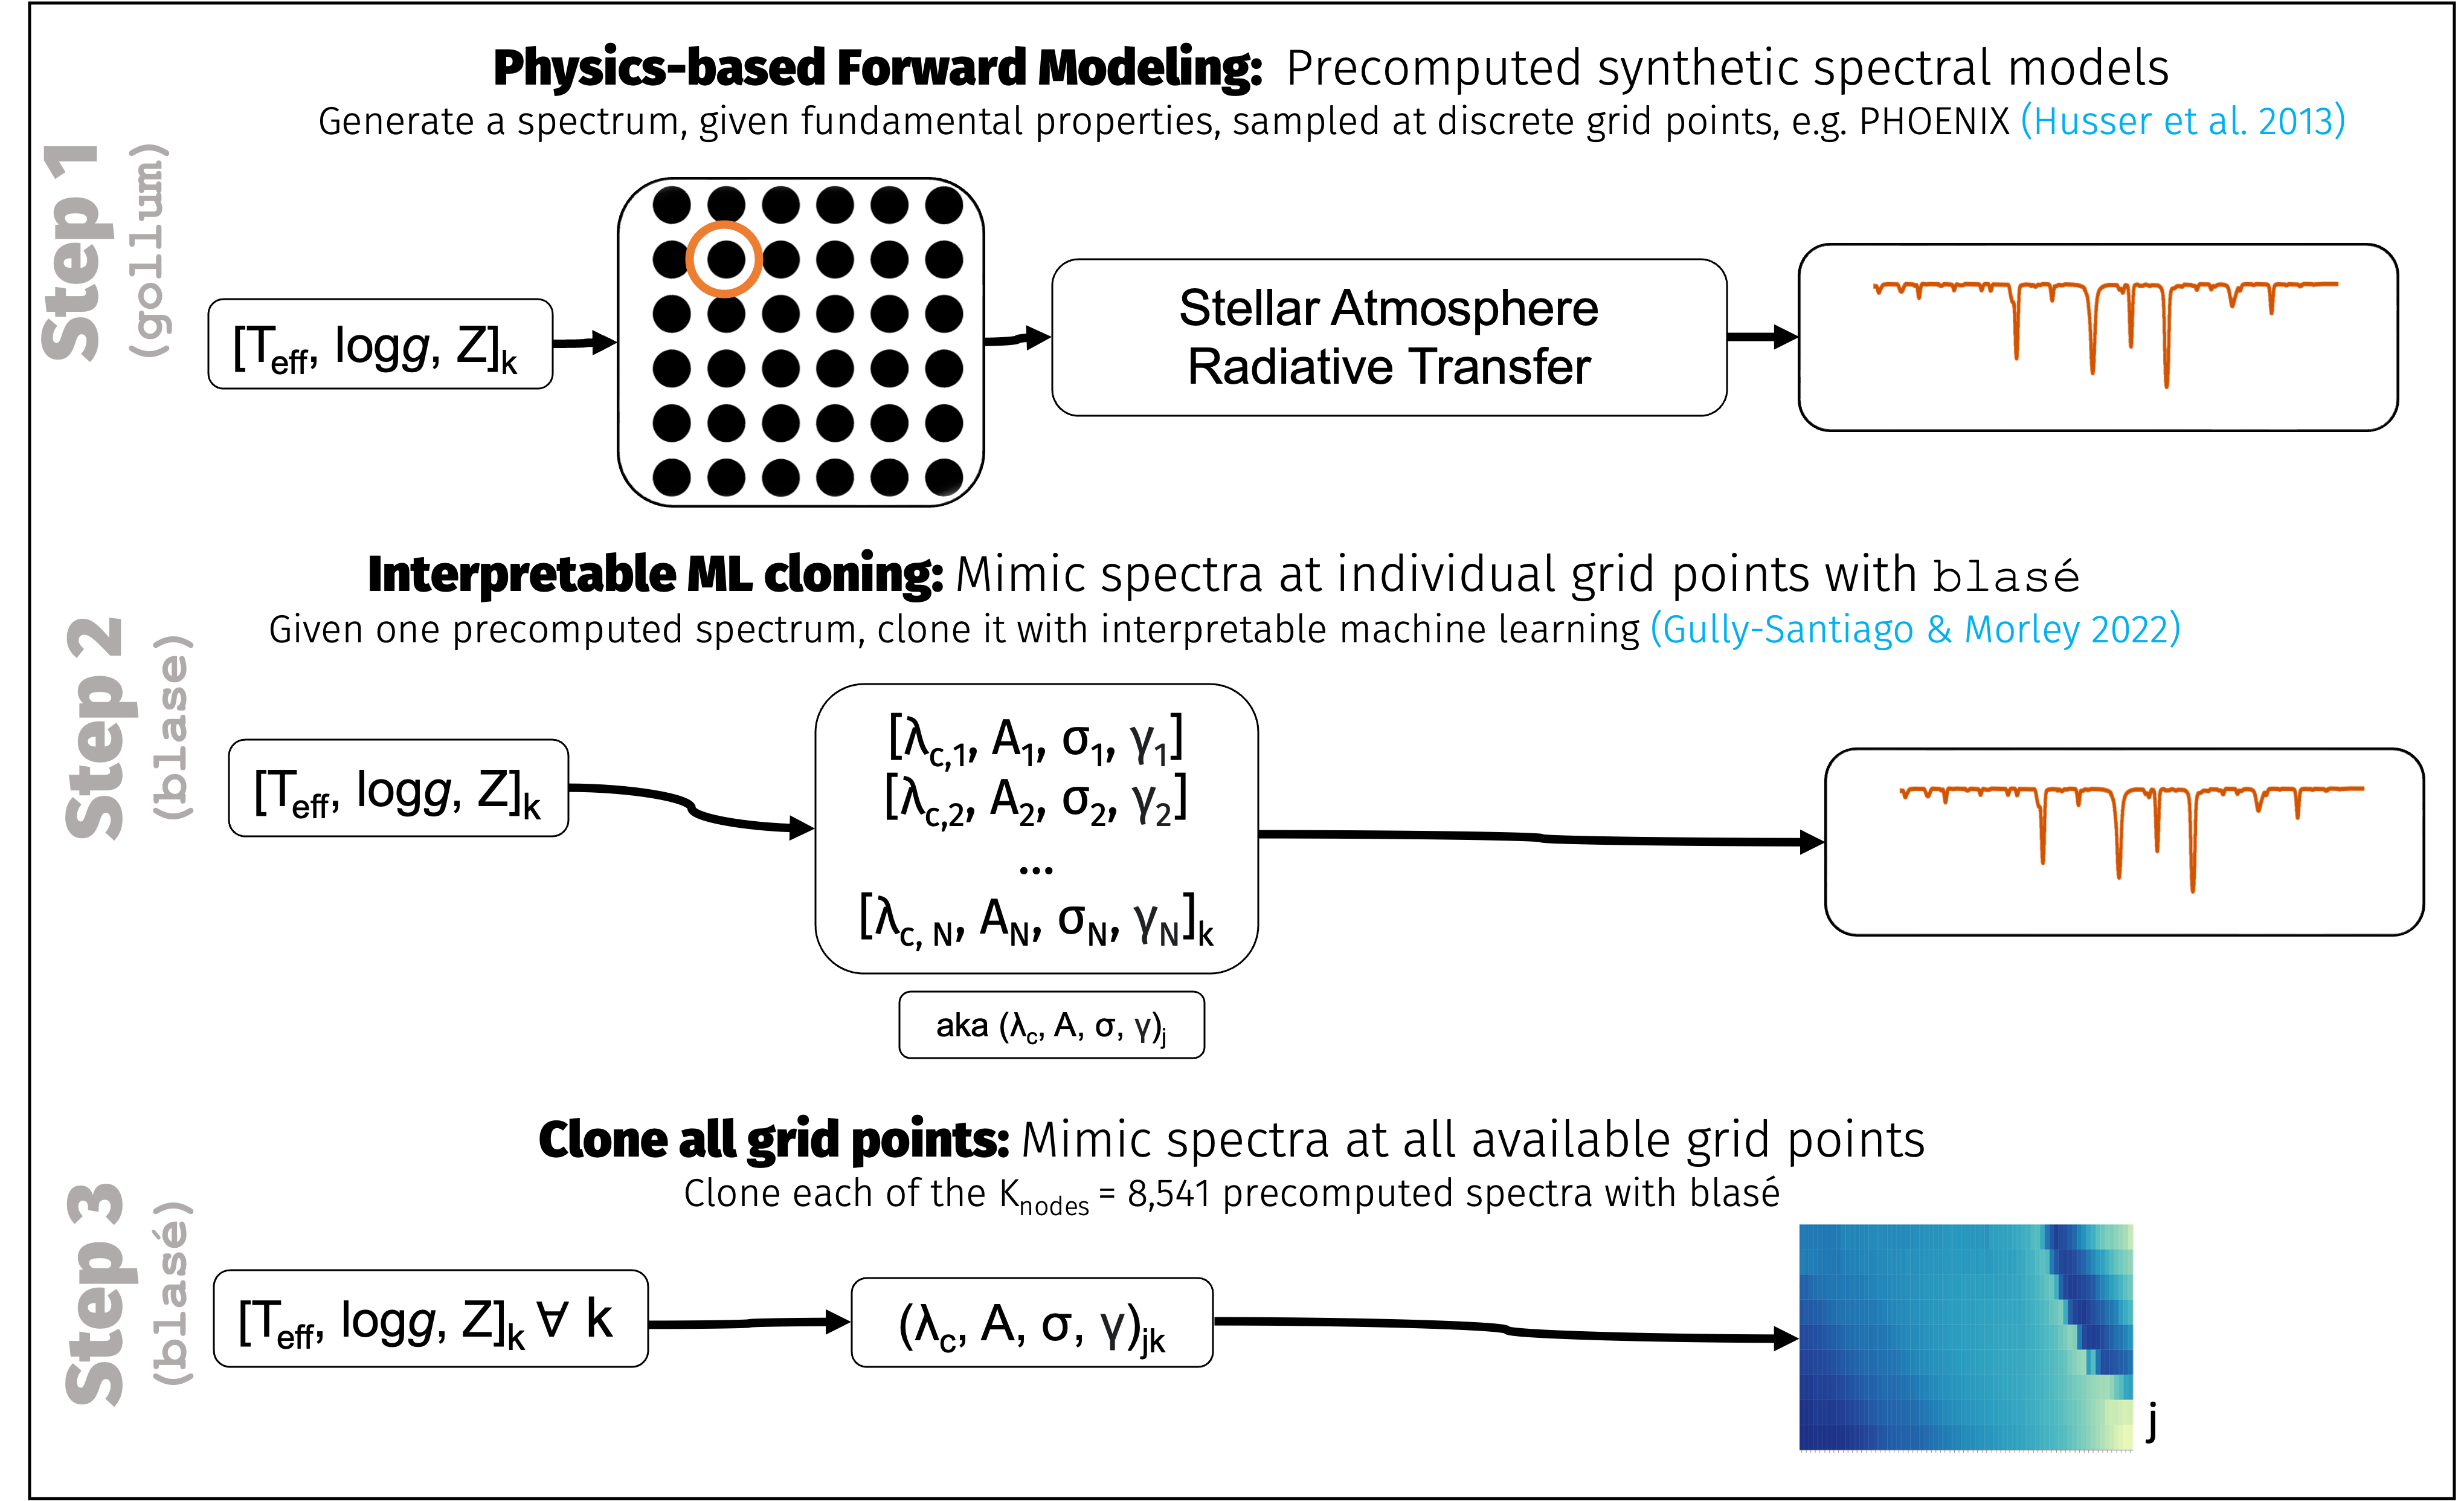
\includegraphics[width=\textwidth]{images/flowchart_frame1_v0p3.png}
    \caption{Flowchart of the cloning steps for emulating precomputed spectra.}
\end{figure*}

\section{Emulating the PHOENIX grid}

For the purposes of this study, we use a slice of the PHOENIX grid where the alpha abundance
is set to zero. Within this slice, we allow the full range of $\Teff, \logg, \Z$. The specific
sampling of the grid points is shown in Figure $XX$. Our approach could feasibly be extended to
include alpha abundances, but given that the \texttt{gollum} interface does not yet support the access
of spectra with nonzero alpha abundances, as well as bearing a significant increase in computational
impact, we leave this for future work.

The \texttt{blase} code takes in any spectrum as input, and outputs a cloned
version of that spectrum. However, there is a hidden product to this
procedure, the state dictionary of the model itself, stored as a \texttt{.pt} file. In this lies metadata about
where spectral lines were identified by \texttt{blase}, as well as those lines'
specific properties, namely amplitude, Gaussian shape, and Lorentzian shape.
In addition, \texttt{blase} also allows the line centers to shift slightly during
cloning, meaning that in addition to the initial line centers, we
also have access to the shifted line centers. This hidden metadata is
what formed the backbone for this study and allowed us to retrieve line-by-line data
that could then be interpolated. We input the PHOENIX grid spectra into \texttt{blase}
and accessed the state dictionaries of each clone. Once this data was retrieved from the state dictionaries
across the grid, it was then aggregated into a single \texttt{pandas} DataFrame, enabling
querying of the data by any property, be it a fundamental stellar parameter or the output
line properties.

All data and code used in this study is available online and is open source. The PHOENIX grid itself takes quite a while to download
due to server bandwidth limitations; this is something that \texttt{gollum} aims to
improve upon by implementing both caching behavior and underlying data structure compression.
\texttt{gollum} itself is available on GitHub and is pip installable, although this
method lags in features significantly compared to the bleeding edge code from GitHub.
\texttt{blase} is the main library of note here, also on GitHub, while the
materials related to this study are currently residing as a fork named \texttt{blase3D}. When polished and complete,
the fork is set to merge into \texttt{blase} itself. Links to all of these are provided in the appendix.

\begin{figure*}
    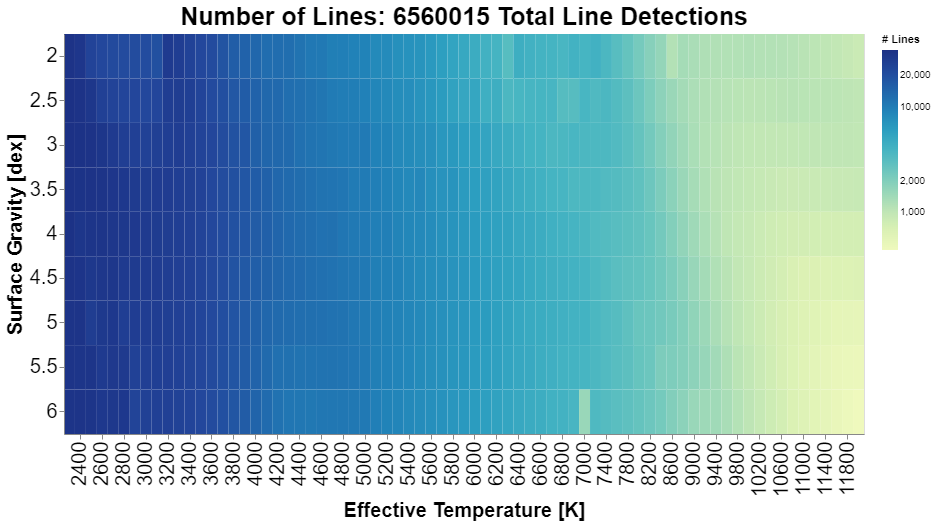
\includegraphics[width=\textwidth]{images/line_density.png}
    \caption{Line density across the grid heatmap}
\end{figure*}


\begin{mdframed}
    \textbf{Figure: Line density across the grid heatmap}
\end{mdframed}


\section{Line-by-Line Fundamental Stellar Properties}
\begin{mdframed}
    \textbf{Conceptual Illustration: Faceted Plot (Teff, Logg, Z) -> Line Profiles}
\end{mdframed}

We have established that the \texttt{blase} code is capable of cloning a spectrum and
returning a set of line properties for each line. In order to visualize line-by-line
properties across the grid, we need to be able to identify unique lines. This begs the question:
what property lets us uniquely identify a spectral line? We have two possible solutions.
First, we consider the shifted line centers. However, this shifting comes from \texttt{blase}'s
emulating physics from its training dataset, meaning that the same line at two grid points could
be shifted differently. Could we then round or truncate the wavelength coordinate of the line centers?
The answer is no, because these shifts vary in precision, and some lines are close enough to begin with
that what should have been two different lines get identified as the same line. This, obviously is incorrect;
one spectral line is just that, one spectral line. So we now consider the original unshifted line centers.
These are the same across the grid, and there is no issue with unintentionally binning lines together
thanks to a uniform precision. This means that we now use the unshifted line centers as the unique
identifier for lines, which vary across the grid in their properties, namely amplitude, Gaussian shape,
and Lorentzian shape.

The next thing that we want to do is to visualize the trends of line properties over
the PHOENIX grid. The best way to visualize this is with heatmaps. This means that for
each line, for each line property, we have one heatmap, where the axes are the fundamental
parameters, and the `temperature' is the value of the line property. As you can imagine, this
is a lot of heatmaps, each of which is incredibly hard to visualize due to the dimensionality.
So, we slice the heatmaps at solar metallicity to reduce them to 2D, and then we can easily
visualize the trend of any one line property of any one line across the grid on demand.

\begin{mdframed}
    \textbf{Figure: Heatmap $\Teff$ vs $\logg$ for a single line $2\times2$ panels for $\sigma$, $\gamma$, $A$, $\lambda$ }
\end{mdframed}

While we see heatmaps for lines that have values at all grid points, this is only true for
a select few spectral lines. The vast majority of lines do not seem to show up at certain
grid points, meaning that our heatmaps are sparse. Initially this seems like it would not be an
issue; when reconstructing, simply retain knowledge of which points were missing and override
the interpolated value with a missing value. Now, in addition to an
interpolator, a sequence of grid points with missing values must be stored for each line just to
override the interpolator. This increases the storage cost of the model. In addition to this, we would
not be able to deal with points lying on the boundary between missing and visible lines. So, we need
to process these missing lines. Since the line properties are on a logarithmic scale,
a line with an amplitude of 0 would have a log amplitude of $-\infty$. This means that we should just
set all missing lines to have log amplitudes of $-\infty$, right? Close, however interpolation
algorithms absolutely despise infinities. So, we set the log amplitude of missing lines to be
$-1000$, which is a large enough negative number that it will effectively evaluate to zero without
causing problems with the interpolation process. We do not really have to worry about the Gaussian
and Lorentzian shape parameters; no matter how `wrong' their interpolated values are, an amplitude of
zero will override that and make the line disappear. This way, we have effectively dealt with
pathological behavior in such a way that interpolation returns a sensible value without sending
the storage impact through the roof.

\section{Mapping Line Parameters to Fundamental Properties}
\begin{mdframed}
    \textbf{Statement: A Bidirectonal Relation exists}
    - Goal: identify a functional form
    \textcolor{lightgray}{\blindtext}
\end{mdframed}

\begin{mdframed}
    \textbf{Figure: Flowchart-with-equations}
\end{mdframed}


\begin{figure*}
    
\includegraphics[width=\textwidth]{images/flowchart_frame2_v0p3.png}
    \caption{Flowchart of the manifold steps for reconstructing a precomputed spectrum.}
\end{figure*}



\begin{mdframed}
    \textbf{Problem: missing lines}
    - Conceivable Solution 1: treat as NaNs and deal with sparsity
    - Conceivable Solution 2: increase model complexity
    \\--------\\
    When using blas\'e, we aggregate the detected lines from all of the grid points
    into one superset of lines. However, not all of the lines in this superset are
    detected at every grid point. In order to deal with this sparsity, we ignore lines
    have $xx$ detections or less. This removes the most sparse lines, but some sparsity still
    remains. The remaining 'missing lines' are dealt with by treating them as Voigt profiles
    with amplitudes of 0, and Gaussian and Lorentzian widths equal to $xx$ and $xx$ respectively.
\end{mdframed}

\section{Performance evaluation}

\begin{mdframed}
    \textbf{Typical Line reconstruction performance}
    \textcolor{lightgray}{\blindtext}
\end{mdframed}

\begin{mdframed}
    \emph{stretch goal}\par
    \textbf{End-to-end PHOENIX grid replication and residual}
    - State the per-pixel residual
    \textcolor{lightgray}{\blindtext}
\end{mdframed}


\section{Discussion}
\begin{mdframed}
    \textbf{Revisiting Model Assumptions}

    \textcolor{lightgray}{\blindtext}
\end{mdframed}

\begin{mdframed}
    \textbf{Functional Form}
    - Describe functional form options and refinement procedures
    - List possibilities, Linreg, GPs \citep{2023ARA&A..61..329A}, NNs, etc.
    - We choose LSTSQ
    - Enumerate functional form
    - Adapting model complexity-- AIC
    \textcolor{lightgray}{\blindtext}
\end{mdframed}

\begin{mdframed}
    \textbf{Limitations}

    - Computational resources
    - Line profile inaccuracy
    - Surface functional form

    \textcolor{lightgray}{\blindtext}
\end{mdframed}

Future studies can expand upon this work in several ways:
\begin{enumerate}[label=-]
    \item Extending the data from just the PHOENIX grid to additional synthetic spectral
          model grids, such as the Sonora substellar model grids or the COOLTLUSTY substellar model grid.
    \item Expanding the section of the PHOENIX grid on which \texttt{blase} was run to include all available alpha abundances, encompassing all of PHOENIX.
    \item Using more advanced regressors with ML techniques to predict line properties instead of using interpolation to brute-force the model predictions.
    \item Extending support to accommodate large-bandwidth spectra across the full electromagnetic spectrum.
    \item Identifying spectral lines using species-based line lists rather than fitting Voigt profiles whenever possible.
\end{enumerate}


\pagebreak
\newpage

\begin{acknowledgments}
    \blindtext
\end{acknowledgments}


\software{}

\bibliography{ms}
\clearpage

\appendix
\section{Notation}
We adopt similar notation to the original blas\'e paper, with some small modifications. We make indexes and
their limits consistent, and remove the use of subscript labeling. We also add new symbols for
wing cut pixels, and radial velocity, as well as introducing three new metrics for reconstruction quality,
storage impact, and computational impact.

\begin{deluxetable}{cp{10cm}}[h]
    \tabletypesize{\small}
    \tablecaption{Notation used in this paper\label{table2}}
    \tablehead{
        \colhead{Symbol} & \colhead{Meaning [former symbol, if applicable]}
    }
    \startdata
    \hline
    \multicolumn{2}{c}{Indexes}\\
    \hline
    $i$ & Pixel index of the precomputed spectrum\\
    $j$ & Spectral line index\\
    $k$ & Grid point index\\
    \hline
    \multicolumn{2}{c}{Spectra}\\
    \hline
    $\bm{\lambda}$ & Spectral axis of the model grid [$\bm{\lambda}_S$]\\
    $\bm{G}$ & The grid of synthetic spectral models\\
    $\mathsf{B}_k$ & Blackbody spectrum of the $k^{th}$ model\\
    $\mathsf{P}_k$ & Continuum polynomial of the $k^{th}$ model\\
    $\mathsf{S}_k$ & Preprocessed flux vector of the $k^{th}$ model\\
    $\mathsf{\hat{S}}$ & Flux vector of the continuous model reconstruction\\
    $\mathsf{R}_k$ & Residual between a $\mathsf{S}_k$ and its reconstruction\\
    \hline
    \multicolumn{2}{c}{Spectral Line Properties}\\
    \hline
    $\mu_{jk}$ & Center position of the $j^{th}$ line in the $k^{th}$ model [$\lambda_c$]\\
    $A_{jk}$ & Amplitude of the $j^{th}$ line in the $k^{th}$ model [$a$]\\
    $\sigma_{jk}$ & Gaussian shape parameter of the $j^{th}$ line in the $k^{th}$ model\\
    $\gamma_{jk}$ & Lorentzian shape parameter of the $j^{th}$ line in the $k^{th}$ model\\
    \hline
    \multicolumn{2}{c}{Scalars}\\
    \hline
    $I$ & Number of pixels in the model grid's spectral axis [$N_x$]\\
    $J$ & Number of spectral lines detected across the grid [$N_{lines}$]\\
    $K$ & Number of grid points in the model grid\\
    $w$ & Wing cut pixel threshold for spectral line identification\\
    $v_r$ & Radial velocity of the star [$RV$]\\
    $R$ & Spectrograph resolving power $\lambda/\delta\lambda$\\
    $Q$ & Quality of a spectral reconstruction\\
    $H$ & The average storage impact of a spectral reconstruction\\
    $Y$ & The average computational impact of a spectral reconstruction\\
    \enddata
\end{deluxetable}

\end{document}

